\documentclass[tikz,border=10pt]{standalone}
\usepackage{tikz}
\usetikzlibrary{calc, intersections}

\begin{document}
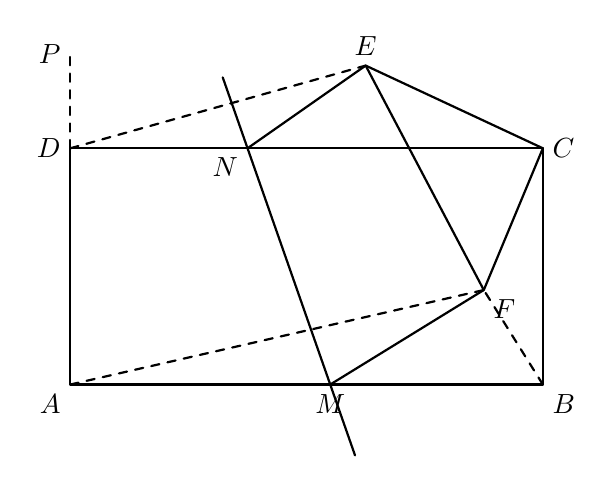
\begin{tikzpicture}[line join=round, line cap=round, >=stealth, scale=1.5]

    % --- 1. 定义核心顶点坐标 (根据视觉比例初步设定) ---
    \coordinate (A) at (0,0);
    \coordinate (B) at (4,0);
    \coordinate (C) at (4,2);
    \coordinate (D) at (0,2);
    
    % --- 2. 定义动点与特定点 ---
    % M 在 AB 上，N 在 CD 上，EF 形成折叠或对称结构
    \coordinate (M) at (2.2, 0);
    \coordinate (N) at (1.5, 2);
    \coordinate (E) at (2.5, 2.7); % 矩形上方的点
    \coordinate (F) at (3.5, 0.8); % 矩形内部/边界的点
    \coordinate (P) at (0, 2.8);   % D点向上的延长线上一点

    % --- 3. 绘制辅助线 (虚线部分) ---
    \draw[dashed, thick] (D) -- (P);      % 左侧向上延伸线
    \draw[dashed, thick] (D) -- (E);      % DE 连线
    \draw[dashed, thick] (A) -- (F);      % AF 连线
    \draw[dashed, thick] (B) -- (F);      % BF 连线

    % --- 4. 绘制实线 (图形主体) ---
    \draw[thick] (A) -- (B) -- (C) -- (D) -- cycle; % 矩形 ABCD
    \draw[thick] (M) -- (N);              % 穿过矩形的斜线 MN
    \draw[thick] (N) -- (E) -- (C);       % 折线 NEC
    \draw[thick] (E) -- (F) -- (M);       % 折线 EFM
    \draw[thick] (C) -- (F);              % CF 连线
    
    % 延伸 MN 的直线部分 (超出矩形边界)
    \draw[thick] (N) -- ($(N)!-0.3!(M)$);
    \draw[thick] (M) -- ($(M)!-0.3!(N)$);

    % --- 5. 标注点名称 ---
    \node[below left] at (A) {$A$};
    \node[below right] at (B) {$B$};
    \node[right] at (C) {$C$};
    \node[left] at (D) {$D$};
    \node[above] at (E) {$E$};
    \node[below right] at (F) {$F$};
    \node[below] at (M) {$M$};
    \node[below left] at (N) {$N$};
    \node[left] at (P) {$P$};

    % --- 6. 装饰 (可选：直角标记等，若题目有要求可添加) ---
    % \draw ($(A)+(0,0.2)$)|-($(A)+(0.2,0)$);

\end{tikzpicture}
\end{document}